\documentclass[11pt,a4paper]{article}
\usepackage[top=3cm, bottom=2cm, left=2cm, right=2cm]{geometry}
\usepackage[utf8]{inputenc}
\usepackage{amsmath, amsfonts, amssymb}
\usepackage{siunitx}
\usepackage[brazil]{babel}
\usepackage{graphicx}
\usepackage[margin=10pt,font={small, it},labelfont=bf, textfont=it]{caption}
\usepackage[dvipsnames, svgnames]{xcolor}
\DeclareCaptionFont{MediumOrchid}{\color[svgnames]{MediumOrchid}}
\usepackage[pdftex]{hyperref}
\usepackage{natbib}
\bibliographystyle{plainnat}
\bibpunct{\textcolor{MediumOrchid}{\textbf{[}}}{\textcolor{MediumOrchid}{\textbf{]}}}{,}{s}{}{}
\usepackage{color}
\usepackage{footnote}
\usepackage{setspace}
\usepackage{booktabs}
\usepackage{multirow}
\usepackage{subfigure}
\usepackage{fancyhdr}
\usepackage{leading}
\usepackage{indentfirst}
\usepackage{wrapfig}
\usepackage{mdframed}
\usepackage{etoolbox}
\usepackage[version=4]{mhchem}
\usepackage{enumitem}
\usepackage{caption}
\usepackage{titlesec}
\usepackage{tcolorbox}
\usepackage{tikz}
\usepackage{LobsterTwo}
\usepackage[T1]{fontenc}
\usepackage{fontspec}
\usepackage{txfonts}
\usepackage[bottom]{footmisc}

\makeatletter
\def\footnoterule{\kern-3pt\color{MediumOrchid}\hrule\@width0.6\textwidth height 0.8pt\kern2.6pt}
\makeatother

\renewcommand{\footnotelayout}{\itshape\color{black}}

\AtBeginEnvironment{equation}{\fontsize{13}{16}\selectfont}


\titleformat{\section}{\LobsterTwo\LARGE\color{CarnationPink}}{\thesection.}{1em}{}
\titleformat{\subsection}{\LobsterTwo\LARGE\color{CarnationPink}}{\thesubsection}{1em}{}


\DeclareCaptionLabelFormat{figuras}{\textcolor{DarkTurquoise}{Figura \arabic{figure}}}
\captionsetup[figure]{labelformat=figuras}

\makeatletter
\renewcommand\tagform@[1]{\maketag@@@{\color{CarnationPink}(#1)}}
\makeatother

\renewcommand{\theequation}{Eq. \arabic{equation}}
\renewcommand{\thefigure}{Fig. \arabic{figure}}
\renewcommand{\thesection}{\textcolor{CarnationPink}{\arabic{section}}}

\setlist[itemize]{label=\textcolor{CarnationPink}{$\mathbf{\square}$}}

\setlist[enumerate]{label=\textcolor{CarnationPink}{\arabic*.}, align=left}


\newcounter{exemplo}

\NewDocumentEnvironment{exemplo}{ O{} }{%
\allowbreak
\setlength{\parindent}{0pt}
  \begin{mdframed}[
  leftline=true,
  topline=false,
  rightline=false,
  bottomline=false,
  linewidth=2pt,
  linecolor=CarnationPink,
  frametitlerule=false,
  frametitlefont=\LobsterTwo\large\color{CarnationPink},
  frametitle={\color{CarnationPink}\LobsterTwo\large #1},
  ]
}{%
  \end{mdframed}
}

\setlength{\fboxsep}{5pt}
\setlength{\fboxrule}{1.5pt}
\usepackage{float}
\renewcommand{\thefootnote}{\alph{footnote}}
\usepackage{url}
\hypersetup{
	colorlinks=true,
	linkcolor=DarkTurquoise,
	filecolor=DarkTurquoise,      
	urlcolor=DarkTurquoise,
	citecolor=DarkTurquoise,
	pdftitle={Especialista em Física da Radioterapia}
}
\pagestyle{fancy}
\fancyhf{}
\renewcommand{\headrulewidth}{0pt}
\rfoot{Página \thepage}

\title{\LobsterTwo\Huge{Radioterapia}}
\author{\LobsterTwo\Large{Planejamento e Métricas Para Determinar a Qualidade do Plano}\nocite{*}}
\date{\LobsterTwo\textit{Dalila Mendonça}}
\begin{document}
	\maketitle

\section{Introdução}

	O objetivo geral do processo de planejamento do tratamento é fornecer a distribuição de dose ideal para o paciente, levando em consideração os seguintes fatores:

	\begin{enumerate}[label=\textcolor{CarnationPink}{(\roman*)}]
		\item Intenção do tratamento (curativo ou paliativo);
		\item Estágio da doença (extensão do envolvimento);
		\item Outras terapias (quimioterapia, hormônios, etc.);
		\item Tratamentos anteriores;
		\item Reprodutibilidade (imobilização, conforto do paciente);
		\item Entregabilidade (colisões, modulação); e
		\item Segurança (sensibilidade a mudanças, robustez).
	\end{enumerate}

	\begin{wrapfigure}{r}{0.4\textwidth}
		\centering
		\fcolorbox{DarkTurquoise}{white}{%
			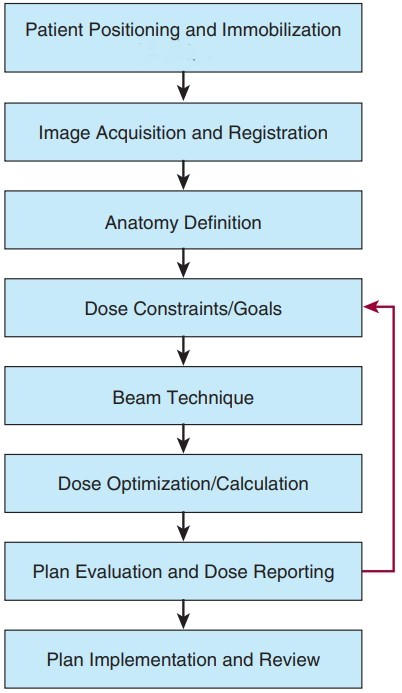
\includegraphics[width=0.3\textwidth]{Imagens/FluxogramadePlanejamento.jpg}
		}%
		\caption{Algoritmo do processo de planejamento.}
		\label{fig:FluxogramadePlanejamento}
	\end{wrapfigure}

	Desde o início, o médico, os técnicos de radioterapia, o físico médico e o dosimetrista devem ter uma comunicação clara sobre os fatores mencionados acima. O máximo de informações possível deve ser documentado no prontuário do paciente para que a sequência de eventos e o status atual do processo de tratamento sejam claros para todos. 
	
	Um esquema do processo de simulação e planejamento do tratamento é mostrado na \ref{fig:FluxogramadePlanejamento}. O fluxo começa com a imobilização e o setup garantindo reprodutibilidade e conforto do paciente. A comunicação é muito importante, como já dito anteriormente. Por exemplo, se um paciente foi submetido a uma cirurgia no ombro e não consegue elevar confortavelmente o braço acima da cabeça, outras estratégias de imobilização podem ser necessárias. Da mesma forma, se um paciente ficar agitado durante a simulação de TC devido à claustrofobia, o técnico precisará se comunicar com o médico e com a enfermagem para que sejam tomadas medidas para reduzir a ansiedade do paciente.

	A capacidade de reproduzir o tratamento de forma confiável ao longo de todo o curso é a chave para a administração bem-sucedida da radioterapia. O primeiro passo para alcançar esse objetivo é um setup e uma imobilização cuidadosa do paciente de modo que maximize o conforto enquanto restringe o movimento.

	Após o posicionamento do paciente, podem ser obtidas imagens que são usadas para definir os alvos e as estruturas críticas necessárias para planejar com segurança o curso do tratamento. Em muitos casos, estudos de imagem adicionais são usados para obter informações sobre a definição de tecidos moles, informações funcionais ou informações metabólicas que não estão disponíveis no conjunto de imagens primário. Esses conjuntos de imagens devem ser co-registrados para preservar a representação geométrica precisa dos dados.

	O contorno preciso do(s) alvo(s) e dos órgãos de risco (OAR) é fundamental para o desenvolvimento de um plano de tratamento de alta qualidade. Se os alvos forem contornados com muita liberdade, os OARs podem receber doses altas desnecessariamente. Da mesma forma, se os OARs forem expandidos em um grau inconsistente com a técnica de setup e localização usada, a dose no alvo pode ser desnecessariamente comprometida.

	

	A intenção médica de tratamento deve conter a dose total planejada e o fracionamento e deve informar as prioridades em relação aos objetivos e restrições de dose. O estágio da doença determinará a extensão da cobertura, como quais cadeias nodais precisam ser cobertas. Mais uma vez, a comunicação é importante. Por exemplo, se o médico disser ao dosimetrista que é aceitável comprometer a cobertura do alvo para garantir que todas os constraints para os OAR sejam atendidos, uma anotação deve ser feita no prontuário para que caso outro dosimetrista assumir o planejamento ou para o físico que revisar o plano também entenda os objetivos utilizados.

	Um plano deve ser consistente com as capacidades do sistema de entrega para que o tratamento seja entregue com segurança. Por exemplo, se for determinado que a reprodutibilidade do setup do paciente e da posição do isocentro é de 3 mm para uma determinada forma de imobilização e para técnica de imagem utilizada, as margens do plano devem refletir essas incertezas (ou seja, não utilizar margens de 1 mm).

	Depois que o contorno estiver finalizado e o método de entrega tiver sido definido, por exemplo, 3D ou radioterapia de intensidade modulada (IMRT), o plano pode ser otimizado. A otimização pode ser um processo manual de tentativa e erro nos casos de entrega conformacional 3D ou um processo de planejamento inverso para as entregas de IMRT. Em ambos os casos, os objetivos de dose desejados devem ser claramente definidos. O responsável pelo planejamento deve estar ciente das limitações do equipamento para evitar a criação de um plano que não pode ser entregue pelo linac. Algumas dessas limitações, como a velocidade do gantry, a taxa de dose, o número mínimo e máximo de unidades monitoras (MU), etc\dots,  podem ser inseridas no sistema de planejamento de tratamento (TPS) para evitar a criação de planos que excedam os limites operacionais do equipamento. Planos com alto grau de modulação podem levar os parâmetros do equipamento ao seu limite e, embora possam ser entregues, podem levar a um excesso de interlocks durante o tratamento.

	Após a otimização do plano, os vários constraints de dose e objetivos de cobertura do alvo são avaliadas para determinar se o plano é aceitável. Caso o plano não seja aceitável, os parâmetros do feixe, como ângulos do gantry ou número de feixes e os objetivos de restrições de dose, podem ser modificados antes de iniciar outra otimização. Pode haver muitas iterações antes que um plano aceitável seja alcançado. Um estudo de Nelms et al. mostrou um amplo grau de variação da qualidade do plano utilizando os mesmos parâmetros de entrada do planejamento. Isso mostra a necessidade de melhores ferramentas para otimizar os planos e o fornecimento orientações a respeito do que é possível ser feito, considerando a anatomia e o diagnóstico exclusivos de um paciente.

\section{Posicionamento e Imobilização}

	Os objetivos da imobilização do paciente incluem:

	\begin{enumerate}[label=\textcolor{CarnationPink}{(\roman*)}]
		\item Reduzir a movimentação do paciente e melhorar a reprodutibilidade diária do posicionamento;
		\item Melhorar o conforto do paciente;
		\item Adaptar às exigências dos dispositivos físicos; e
		\item Evitar entradas de campos em tecidos normais.
	\end{enumerate}

\section{Aquisição e Registro de Imagens}

	A tomografia computadorizada (TC) é a principal modalidade de imagem na radioterapia. A TC nem sempre produz o melhor contraste de tecidos moles para o delineamento de órgãos de risco e dos alvos, mesmo com o uso de agentes de contraste. Atualmente, a TC é necessária para os cálculos de dose dos planejamento do tratamento com precisão porque é a única modalidade de imagem que fornece informações de densidade e, portanto, de atenuação.
	
	Os materiais de alta densidade, como próteses de quadril e implantes dentários, podem causar artefatos ``streaking'' significativos. Estes artefatos podem causar dificuldade na identificação dos alvos e dos órgãos de risco. O impacto desses artefatos no cálculo da dose é mínimo nos casos de próteses de quadril, mas tem mostrado um impacto significativo nos casos de obturações dentárias. Nesses casos uma imagem de ressonância magnética (RM) pode ser útil. Caso disponível, a TC de megavoltagem (MVCT) pode ser usada para reduzir os artefatos devido à diminuição do efeito fotoelétrico em energias mais altas.
	
	Os tomógrafos mais novos têm a capacidade de reconstruir dados fora do feixe em leque primário de modo que seja possível criar um campo de visão expandido (FOV). Esta técnica pode ajudar a contornar todo o contorno externo do paciente. Entretanto, a densidade nas áreas expandidas tem se mostrado imprecisa e deve-se ter cuidado ao usá-la para planejamento.

	A tomografia por emissão de pósitrons (PET)/TC é frequentemente usada para obter informações metabólicas que indicariam a atividade do tumor. As varreduras levam um tempo relativamente longo para serem adquiridas, envolvem o uso de material radioativo, têm baixa razão sinal-ruído em alguns casos e têm baixa resolução espacial. O uso do PET/CT depende do uso de protocolos de aquisição, reconstrução e segmentação de imagens bem definidos.

	Alguns pesquisadores estão trabalhando em metodologias para correlacionar os sinais da RM com a densidade do meio. Caso isso puder ser feito, a RM poderia ser usada como única modalidade de planejamento, o que permitiria aproveitar a definição superior dos tecidos moles fornecidos pela RM, bem como eliminar o uso de radiação ionizante para aquisição das imagens de planejamento. A ressonância magnética pode ser usada para delinear tecidos moles, obter informações metabólicas e funcionais dos órgãos e tumores e para monitorar a resposta ao tratamento, o que aproveitaria da falta de dose de radiação e, portanto, podem ser feitos exames com segurança em uma frequência mais alta. Em alguns casos, a espectroscopia com prótons pode ser usada para identificar malignidades ou tecidos necróticos. Contudo, as desvantagens da simulação do tratamento utilizando RM seria a precisão geométrica potencialmente menor, o FOV menor, os tempos de aquisição muito mais longos e custo mais elevado.

	O uso de duas ou três modalidades de imagem para um único paciente não é incomum porque as modalidades têm pontos fortes diferentes. Combinar com precisão essas imagens para obter uma imagem anatômica, metabólica e funcional completa requer um processo de registro preciso. Isso pode ser particularmente desafiador se algumas das imagens não forem feitas com o paciente na posição de tratamento.
	
	Os algoritmos de registro de imagem são classificados como rígidos ou deformáveis:

	\begin{itemize}
		\item O \textcolor{DarkTurquoise}{\textbf{registro rígido}} se trata de uma translação geométrica simples com a rotação de um conjunto de imagens para alinhar uma com as outras. Esta modalidade não consegue levar em conta as diferenças na posição ou movimentação do paciente.
		
		\item O \textcolor{DarkTurquoise}{\textbf{registro deformável}} mapeia um conjunto de imagens em outro conjunto de imagens usando uma matriz de transformação para produzir um mapa de deformação. Esta modalidade permite o registro de de imagens contendo diferenças no posicionamento do paciente, na movimentação do paciente e alterações no tamanho e na forma do órgão.
	\end{itemize}

	A validação do registro deformável é muito complexa. O AAPM TG-132, \textcolor{MediumOrchid}{\textit{``Use of Image Registration and Data Fusion Algorithms and Techniques in Radiotherapy Treatment Planning''}}, está desenvolvendo um report que revisará os algoritmos de registro deformável existentes e discutirá questões relacionadas à implementação, métodos de avaliação da precisão do registro, questões relacionadas ao teste de aceite e controle de qualidade (QA). Várias publicações analisaram a precisão de diferentes algoritmos. Em geral, nenhum algoritmo funciona com a mesma precisão em todas as situações e, portanto, eles devem ser avaliados em cada aplicação clínica.

\section{Definição Anatômica}

	A definição das estruturas anatômicas é crucial para alcançar a entrega da radioterapia com alta qualidade. O contorno dos alvos de tratamento e dos OARs pode ser um processo demorado, como ocorre por exemplo em casos de IMRT de cabeça e pescoço, ou podem ser relativamente simples como ocorre nos casos de tratamentos paliativos da coluna. 

	Quanto à padronização das estruturas dos reports do tratamento, dois importantes reports são:

	\begin{enumerate}
		\item \textcolor{DarkTurquoise}{\textbf{ICRU-83}} - Prescribing, Recording, and Reporting Photon-Beam Intensity-Modulated Radiation Therapy (IMRT); e
		\item American Society for Radiation Therapy (ASTRO) 2009 Recommendations for Documenting IMRT 
		Treatments.
	\end{enumerate}

	Embora esses relatórios mencionem especificamente IMRT em seus títulos, eles também se aplicam a outras técnicas. A AAPM lançou em 2018 o report do TG-263, Standardizing Nomenclature in Radiation Oncology, que fornece os guidelines para a padronização das nomenclaturas utilizadas na Radioterapia. 

	As estruturas descritas na \ref{fig:estruturasIcru83} são uma modificação e atualização do ICRU-50 e ICRU-62, que definiram esses conceitos. As recomendações do relatório para IMRT de 2009 da ASTRO exigem que o médico especifique todos os volumes da \ref{fig:estruturasIcru83}, exceto os volumes RVR e TV, que são estruturas de planejamento.

	\begin{figure}[h]
		\centering
		\fcolorbox{DarkTurquoise}{white}{%
			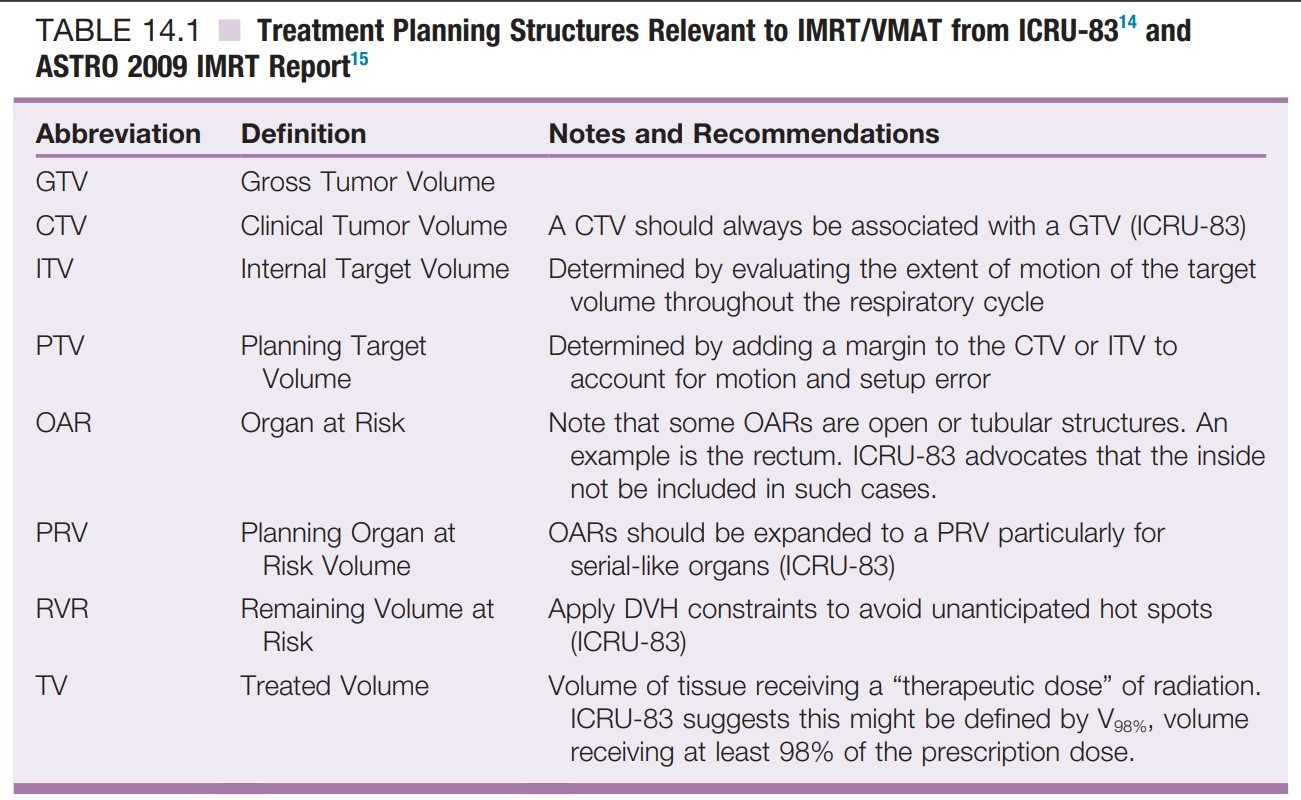
\includegraphics[width=0.8\textwidth]{Imagens/estruturasIcru83.jpg}
		}%
		\caption{Estruturas de planejamento de tratamento relevantes para IMRT/VMAT definidas no ICRU-83.}
		\label{fig:estruturasIcru83}
	\end{figure}

	Em alguns sistemas de planejamento, o processo de delineamento começa com o delineamento do contorno  externo do paciente (body), embora nem todos os sistemas de planejamento exijam essa estrutura. Alguns sistemas fazem o contorno do body automaticamente ao importar a imagem. Nesses casos,  o contorno do body deve ser avaliado para determinar sua precisão, pois essa estrutura determinará a profundidade do tratamento e, finalmente, a MU. As áreas típicas que requerem atenção no contorno do body são as áreas ao redor da boca e do nariz, onde o contorno pode ficar dentro do corpo, ou pode englobar fios ou marcadores colocados na pele além dos dispositivos de imobilização. 

	A maioria dos sistemas de planejamento não leva em consideração qualquer estrutura que estiver fora do contorno corporal (fora do body) e, portanto, os acessórios de imobilização deverão ser contornados e considerados como parte do corpo, caso o impacto dosimétrico desses acessórios deva ser calculado. Alguns sistemas têm a capacidade de adicionar a mesa de tratamento ao conjunto de imagens para contabilizar adequadamente a atenuação no tampo da mesa.

	Alguns sistemas de planejamento (como por exemplo o TomoTherapy e o Pinnacle) consideram cada estrutura dentro do FOV de aquisição e, portanto, calculam inerentemente a atenuação dos dispositivos de imobilização. Um cuidado ao usar um sistema com essa capacidade é que alguns artefatos de imagem da TC criam um anel brilhante ao redor da borda do FOV, que será visto como uma região de alta densidade pelo TPS e a MU será aumentada artificialmente. A avaliação cuidadosa do conjunto de imagens deve ser feita diminuindo o zoom para mostrar o FOV máximo e alternando para uma janela de pulmão para tornar o anel formado mais óbvio. Alguns TPSs têm a capacidade de filtrar artefatos de baixa densidade fora do contorno do corpo aplicando um valor de threshold.

	O contorno dos alvos é feito pelo médico, que normalmente contornará um GTV ou CTV. O dosimetrista ou físico pode então criar um PTV usando critérios de expansão especificados pelo médico. O médico pode ser auxiliado no delineamento do alvo por meio do uso de um algoritmo de segmentação baseado em atlas que usa registro deformável de um caso “especializado”. Os contornos finais devem ser cuidadosamente revisados e modificados conforme necessário pelo médico.

	O contorno dos OARs é normalmente feito por dosimetristas e médicos. Os dosimetristas geralmente contornam a anatomia óssea, medula espinhal, pulmão e outras estruturas facilmente identificáveis, como rins e fígado. Isso pode ser feito usando técnicas manuais, segmentação baseada em atlas, segmentação automática ou segmentação baseada em modelos. A segmentação automática depende de seguir os limites de densidade e exige que o usuário coloque um ponto de origem ou volume delimitador. Eles funcionam bem para órgãos com alto contraste em relação ao tecido circundante, como o pulmão. Os algoritmos de segmentação baseados em modelo têm as propriedades típicas de um órgão relacionadas ao tamanho, forma e densidade que são usadas para determinar os contornos. Eles também podem usar um ponto de origem ou volume delimitador. Novamente, esses contornos automatizados devem ser revisados e modificados conforme necessário.

	O contorno impreciso pode levar a planos abaixo do ideal, atrasar o processo de planejamento pois torna difícil ou impossível atingir algumas metas de dose ou então pode causar erros geográficos (erros no posicionamento). O contorno preciso do alvo e dos OARs são essenciais para um planejamento de alta qualidade. A importância do contorno correto é enfatizada no report da ASTRO \textbf{\textit{``Safety Is No Accident''}} e no white paper de segurança a respeito da revisão por pares, no qual o papel da revisão por pares dos contornos é enfatizado. Deve-se reconhecer que, se os contornos só forem revisados depois do planejamento, o limite para rejeição será muito maior porque o processo de planejamento terá que ser repetido. Isso levou alguns grupos a explorar a revisão por pares antes do planejamento, e isso é defendido no report  S\textbf{\textit{``Safety Is No Accident''}}. Alguns atlas de contorno estão disponíveis para auxiliar no delineamento dos volumes. O NRG Oncology tem um atlas de contorno disponível em seu site, bem como links para o atlas do Radiation Therapy Oncology Group (RTOG), Gynecologic Oncology Group (GOG) e National Surgical Adjuvant Breast and Bowel Project (NSABP) em \href{http://www.nrgoncology.org/Resources.aspx}{http://www.nrgoncology.org/Resources.aspx}. As definições de CTV em atlas, por exemplo, podem variar de acordo com o estágio.

	Um parâmetro crucial no planejamento é a margem usada para expandir do CTV para o PTV. Uma margem muito pequena resulta em um risco de subdosar o CTV. No entanto, se fosse necessária uma cobertura dosimétrica do CTV de 100\% em todos os pacientes, seria necessária uma margem muito grande do CTV para o PTV, resultando em doses mais altas nos OARs. É evidente que algum comprometimento da cobertura é necessário. Uma solução para esse problema vem na formulação de ``regras para margens''.

\section{Margens}

	As formulações de regras para margens datam de pelo menos 1995 e estão bem resumidas na Tabela 4.4 do ICRU-83, apresentada na \ref{fig:margensIcru83}. O conceito básico é que, com informações sobre a variabilidade do posicionamento em uma população de pacientes, pode-se calcular a margem necessária para garantir a cobertura dosimétrica em, digamos, 90\% dos pacientes. A Tabela 4.4 do ICRU-83 lista 11 fórmulas de determinação da margem para cálculos de expansão do CTV para PTV ou do OAR para PRV. Talvez a fórmula mais utilizada seja a de van Herk et al. onde a regra para a margem é de $2.5\sum + 0.7\sigma$, onde $\sum$ e $\sigma$ são as incertezas sistemáticas e aleatórias, respectivamente, no posicionamento do paciente. $\sum$ e $\sigma$ devem ser medidos para cada clínica a partir dos dados obtidos através da radioterapia guiada por imagem (IGRT) ou a partir de outros dados. Esta fórmula baseia-se no objetivo de atingir uma dose mínima de cobertura no CTV de 95\% para 90\% dos pacientes. Essa fórmula de margem determinada através da população é baseada na suposição de que o plano é perfeitamente conformado. Essa formulação também assume algo sobre a penumbra do feixe, embora esteja disponível uma fórmula mais generalizada que considera explicitamente a largura da penumbra.

	\begin{figure}[h]
		\centering
		\fcolorbox{DarkTurquoise}{white}{%
			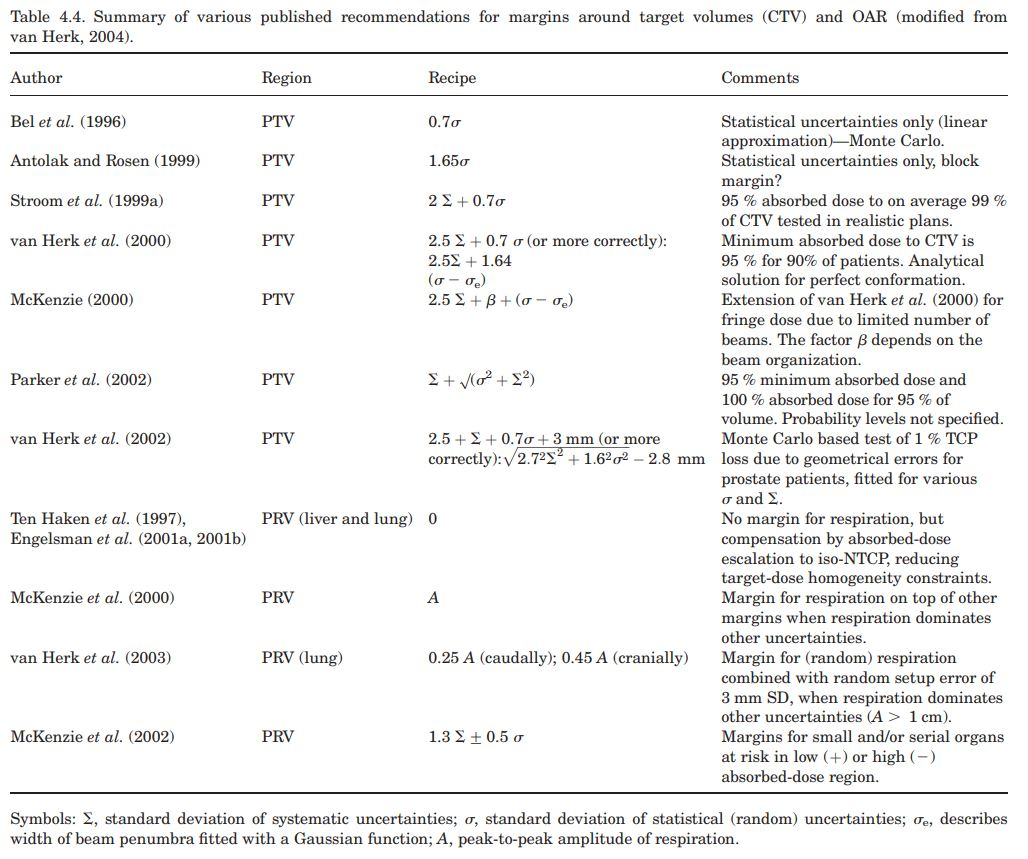
\includegraphics[width=0.6\textwidth]{Imagens/margensIcru83.JPG}
		}%
		\caption{Margin recipe formulations.}
		\label{fig:margensIcru83}
	\end{figure}
	

	É importante reconhecer que as fórmulas de margem simplificadas mencionadas acima foram desenvolvidas sob as suposições de que a radioterapia conformada 3D está sendo usada e que a estatística de Poisson será usada para o fracionamento padrão. Estes podem não ser aplicáveis para planos de IMRT, que possuem diferentes conformidades e gradientes de dose ou cursos hipofracionados nos quais o número de frações é menor. Um estudo de casos de cabeça e pescoço encontrou margens três vezes menores do que seria sugerido pela formulação de van Herk et al. A implicação é que as margens podem precisar ser diferentes para tratamentos IMRT.

	Independentemente da fórmula adequada, deve-se reconhecer que o uso de IMRT sozinho geralmente não garante uma redução nas margens. A técnica de IMRT tem mais impacto em gradientes de dose, o que pode resultar em menos dose para os OARs próximos, mas não afeta a variação do setu, que a margem foi projetada para mitigar. A redução da margem é alcançada de forma mais adequada por meio do uso de IGRT em vez de IMRT. De fato, um estudo demonstrou aumento da falha bioquímica em pacientes de próstata com redução inapropriada da margem. Nesse contexto, também é importante observar que uma fórmula de margem como $2.5\sum + 0.7\sigma$ sugere que a componente sistemática da variabilidade ($\sum$) é aproximadamente 3 vezes mais importante que a componente variabilidade aleatória ($\sigma$). Se as margens devem ser reduzidas, é particularmente importante abordar a componente sistemática da variabilidade e portanto o IGRT é particularmente eficaz em realizar essa redução.

	As margens a serem usadas para gerar o PTV devem ser definidas pelo médico em consulta com o físico médico. Isso pode ser feito caso a caso ou como uma solução de classe (por exemplo, pacientes com câncer de próstata recebendo 80 Gy em três fases, com cada fase usando um conjunto diferente de margens). As margens podem ser determinadas localmente com base na análise de variações de setup ou com base em recomendações publicadas. Caso utilizar recomendações publicadas, o usuário deve verificar o uso de uma metodologia IGRT apropriada em comparação com o que foi usado no estudo publicado.

	Outro fator a ter em mente é que o volume tratado (volume englobado pela isodose de prescrição, TV) em geral não corresponde ao PTV gerado por qualquer fórmula de margem. O TV geralmente toca o PTV em algumas áreas e geralmente é maior que o PTV, embora em alguns casos o TV possa ser menor que o PTV caso as restrições dos OARs tiverem prioridade sobre a cobertura do PTV.

\section{Constraints e Objetivos}

	O objetivo da otimização é maximizar a dose nos alvos enquanto minimiza a dose nos OARs. Em muitos casos, a dose total nos alvos é limitada pelas doses de tolerância dos OARs. O estabelecimento de constraints de dose confiáveis tem sido um desafio em Radioterapia. A ASTRO  e a AAPM desenvolveram o \textbf{\textit{``Quantitative Analysis of Normal Tissue Effects in the Clinic (QUANTEC)''}} publicado no \textit{International Journal of Radiation Oncology Biology and Physics} em março de 2010 e também está disponível no site da AAPM, \href{http:// aapm.org/pubs/QUANTEC.asp}{http:// aapm.org/pubs/QUANTEC.asp}. Toda esta edição da revista é dedicada ao tema e inclui artigos específicos sobre 16 órgãos de risco. A \ref{fig:quantec} é adaptada do QUANTEC, que descreve os dados para o fracionamento padrão (1.6 a 2.0 Gy/fração, uma ou duas vezes ao dia).

	\begin{figure}[h]
		\centering
		\subfigure{
			\fcolorbox{DarkTurquoise}{white}{%
				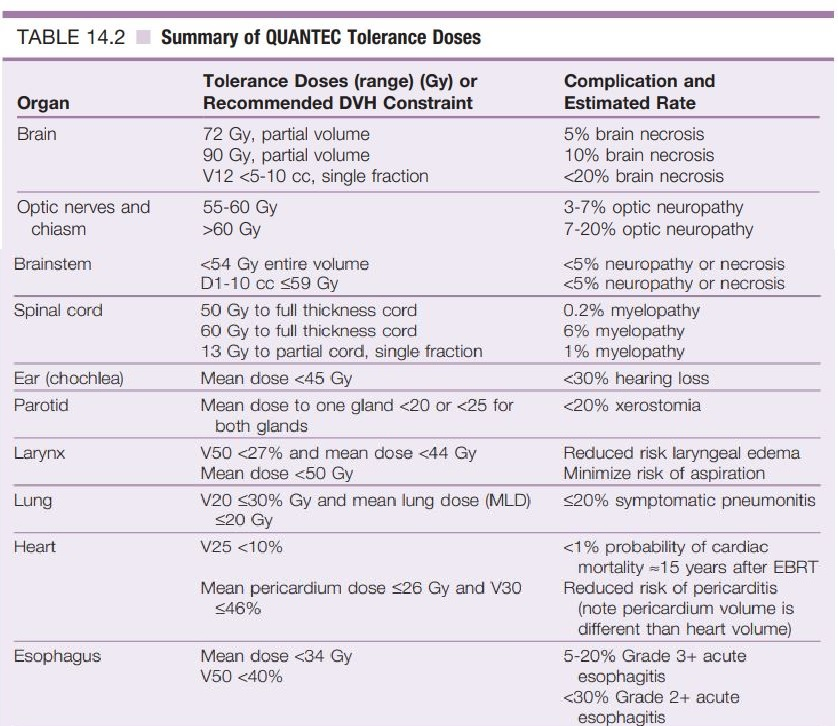
\includegraphics[width=0.45\textwidth]{Imagens/quantec1.JPG}
			}} %
			\subfigure{
			\fcolorbox{DarkTurquoise}{white}{%
				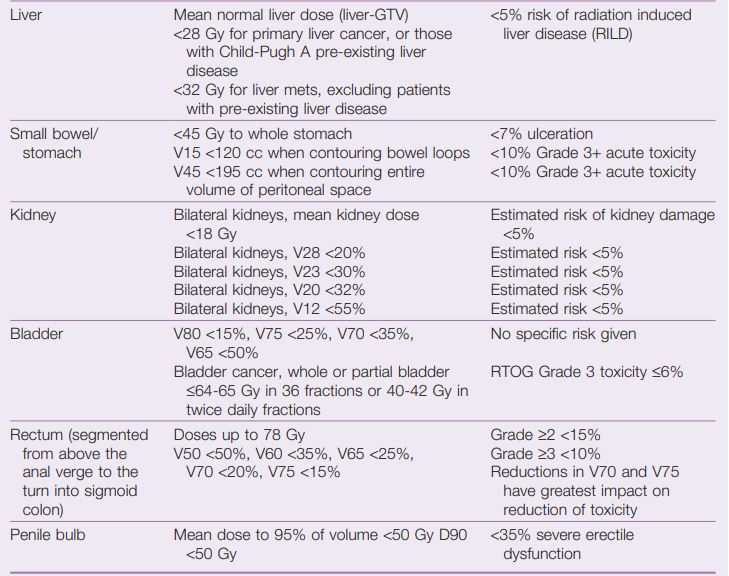
\includegraphics[width=0.45\textwidth]{Imagens/quantec3.JPG}
			}} %
		\caption{QUANTEC}
		\label{fig:quantec}
	\end{figure}

	Embora esses números sejam compilados a partir dos relatórios do QUANTEC, existem muitos fatores que afetam os constraints de dose, como tamanho da fração, dose total, volume de tecido e combinação com quimioterapia. Portanto, o leitor é aconselhado a ler todo o relatório QUANTEC, incluindo os capítulos específicos de cada órgão, antes de adotar um constraint de dose no caso clínico. Ensaios clínicos randomizados geralmente incluem limites de dose e são outra boa fonte de dados. Deve-se observar que antes de adotar uma restrição de dose para uso na clínica, deve-se entender a taxa de complicações do constraint adotado. Embora uma taxa de complicação de 10\% possa ser aceitável para alguns médicos em algumas circunstâncias, pode não ser para outros. 

\section{Técnicas de Tratamento}

	Após os contornos terem sido delineados e revisados, os feixes podem ser inseridos. Isso pode ter sido feito durante o processo de simulação (o que é raro hoje em dia). Existem muitas técnicas de tratamento possíveis (por exemplo, campos únicos, múltiplos feixes fixos com conformacionais, campo em campo, múltiplos feixes com IMRT, campos de arcos conformacionais, campos VMAT ou uma combinação destes citados). Como os tratamentos evoluíram de 3D conformacional, para IMRT e depois para VMAT, houve mudanças distintas na natureza das distribuições de dose resultantes. Cada técnica tem vantagens e desvantagens, mas a situação clínica determinará qual será técnica será utilizada. A comunicação entre os membros da equipe é crucial para esta definição. Em última análise, o planejador provavelmente tentará várias abordagens para encontrar o melhor plano aceitável.

	No \textcolor{DarkTurquoise}{\textbf{planejamento 3D tradicional}}, um número limitado de feixes fixos é utilizado, normalmente na ordem de 3 a 5 feixes. Os vários parâmetros são ajustados manualmente para produzir um resultado aceitável. Geralmente, é alcançada uma dose homogênea em todo o alvo. O feixe pode ser conformado usando filtros ou técnicas de field-in-field. Com o advento dos feixes sem filtro aplanador (FFF - \textit{ flattening filter free}), isto também pode ser obtido usando um meio campo bloqueado no feixe FFF, pelo menos no caso de campos tangentes de mama onde um feixe cilindricamente simétrico é útil.

	O advento da \textcolor{DarkTurquoise}{\textbf{técnica de IMRT}} trouxe o conceito de planejamento inverso, no qual pequenos segmentos de feixe são otimizados para atingir os objetivos de dose desejados. Isso geralmente resulta em uma cobertura de alvo muito heterogênea com pontos quentes concentrados em um local. A otimização IMRT é capaz de produzir gradientes de dose mais acentuados em algumas direções para poupar melhor os OARs. Além disso, podem ser criadas distribuições côncavas envolvendo a dose ao redor da medula espinhal, por exemplo. A técnica de IMRT demonstrou poupar melhor os OAR à custa de um maior volume de tecido exposto a baixas doses.

	A \textcolor{DarkTurquoise}{\textbf{técnica de VMAT}} tem a vantagem de otimizar a distribuição de todas as direções do arco. Embora isso dê ao otimizador mais flexibilidade em alguns aspectos, pode ser uma desvantagem se houver alguns ângulos discretos que tenham uma geometria mais ideal. A técnica de VMAT também distribui as doses baixas em um volume ainda maior. Um estudo mostrou um aumento de até 11\% na dose total usando uma abordagem VMAT versus IMRT com campo fixo.

	Há um debate quanto ao significado das diferenças na dose integral entre os métodos. Uma m,maior dose integral levará a mais cânceres secundários? Um estudo demonstrou um risco aumentado com doses integrais mais altas. Uma publicação recente revisou a literatura e determinou que mais estudos de longo prazo eram necessários antes que qualquer conclusão pudesse ser tirada. Em geral, é sempre uma boa prática minimizar a dose fora do volume irradiado para reduzir o risco de cânceres secundários.

\section{Otimização e Cálculo de Dose}

	A otimização de dose pode ser um processo manual de tentativa e erro através da manipulação de ângulos de feixe, ângulos de colimador, ângulos de mesa, pesos dos campos, modificadores de feixe e energia do feixe. Desde meados da década de 1990, algoritmos automatizados para IMRT estão em uso. Mais comumente chamado de planejamento inverso, o processo envolve o planejador definindo os objetivos de dose desejados para os alvos e para os OARs. As Funções objetivo e as prioridades são usadas pelo algoritmo para determinar quais objetivos enfatizar durante a otimização.
	
	Uma função objetivo descreve o custo para exceder um objetivo de dose para um OAR ou não atingir um objetivo de dose para um alvo. As funções podem ter limites (ou seja, a medula não deve exceder 5.000 cGy), funções lineares (risco proporcional à dose), funções exponenciais (quando a dose excede um certo nível, o risco se torna muito maior) ou muitas outras possibilidades. Estas também são conhecidas como funções de custo. Modelos biológicos podem ser usados no processo de otimização. Esses modelos tentam explicar as diferentes respostas biológicas dos tecidos à dose física entregue.

	Deve-se observar que os valores de dose e os parâmetros definidos no processo de otimização não são iguais aos objetivos clínicos desejados, mas muitos sistemas TPS não têm como distinguir entre os dois. Durante o processo de otimização, os valores de dose para um OAR ou alvo podem ser ajustados para um valor artificialmente maior ou menor na tentativa de direcionar a otimização para o resultado desejado. O plano ainda deve ser avaliado usando os objetivos originais. Se o TPS não tiver a capacidade de diferenciar entre objetivos de planejamento e valores de otimização, deve ser claramente documentado que esse é o caso.

	Depois que um plano foi otimizado e está pronto para revisão médica, é aconselhável que o plano seja submetido a uma revisão por pares para confirmar sua integridade. Um estudo descreveu um método automatizado para verificar a integridade do plano antes de ser apresentado ao médico para aprovação. \citet{yang2012automated} desenvolveu scripts e módulos de software que verificam automaticamente uma grande variedade de informações do plano. Um resumo da Tabela I deste report é mostrado na \ref{fig:checkPlanoAutomatizado}. Os itens desta tabela devem ser verificados usando um método automatizado conforme descrito ou um método manual como foi feito nesta instituição antes de desenvolver o processo automatizado.

	\begin{figure}[h]
		\centering
		\fcolorbox{DarkTurquoise}{white}{%
			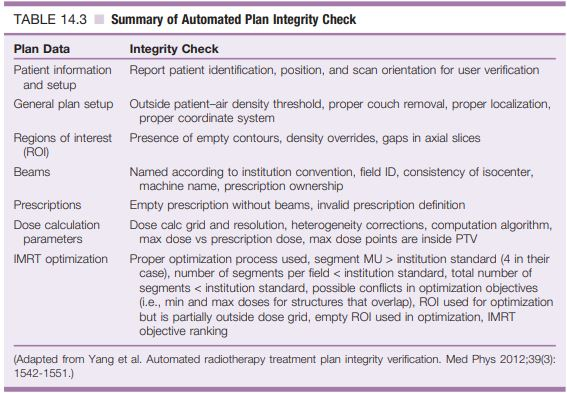
\includegraphics[width=0.7\textwidth]{Imagens/checkPlanoAutomatizado.JPG}
		}%
		\caption{Resumo da Verificação Automatizada da Integridade do Plano.}
		\label{fig:checkPlanoAutomatizado}
	\end{figure}

\section{Avaliação do Plano e Report da Dose}

	Tanto o ICRU-83 quanto o report da ASTRO defendem fortemente o report da dose baseado em DVH, em vez de reportar a dose para o(s) ponto(s). Isso é necessário para comparar um plano específico com os reportes publicados de constraints dos tecidos normais, como por exemplo, os reports do QUANTEC. Isso evita uma possível falha em reportar a dose para um ponto específico, porque esse ponto pode ser uma dose baixa ou alta, dependendo de onde este ponto está localizado no volume. O report 2009 sobre IMRT da ASTRO observa que, se a prescrição de dose pontual for usada, a diferença entre a dose real administrada e a dose prescrita pode variar em mais de 10\%. Por esse motivo, deve-se ter cuidado ao interpretar os registros de tratamento realizados em outra instituição caso as métricas de DVH não forem reportadas.

	A estatística DVH mais relevante é o valor $D_{V\%}$. Por exemplo,  $D_{100\%}$ do PTV é a dose mínima recebida por 100\% do volume do PTV. Alternativamente, isso pode ser declarado como um valor $V_{D_{Gy}}$ (ou seja, o percentual de volume ou o volume absoluto de um órgão que recebe uma dose de D Gy ou mais). Não há nenhuma recomendação rígida no ICRU-83 sobre qual valor de $D_{V\%}$ deve ser reportado para as estruturas-alvo. O relatório observa, porém, que $D_{50\%}$ do PTV parece ser mais consistente em todos os sistemas de planejamento. O ICRU-83 recomenda que, se$D_{50\%}$ não for usado para definir a prescrição, pelo menos seja relatado. O relatório ASTRO 2009 IMRT vai um pouco mais longe, recomendando que as seguintes doses sejam relatadas tanto para o PTV quanto para o CTV: dose média, $D_{95\%}$, $D_{100\%}$, $V_{100\%}$ e a dose máxima. O report recomenda que, no mínimo, seja anotada a dose prescrita (e seu fracionamento) e o ponto ou volume para o qual a dose é prescrita.

	Para OARs, o relatório ASTRO 2009 IMRT recomenda que as seguintes doses sejam relatadas: dose máxima, dose mínima e dose média. O ICRU-83 é um pouco mais específico e recomenda que uma estatística de dose “quase-máxima” ou “quase-mínima” seja usada. Um exemplo seria $D_{2\%}$ (a dose recebida por 2\% ou mais dos OAR) e $D_{98\%}$ (a dose recebida por 98\% ou mais dos OAR). Estas são mais confiáveis do que as doses pontuais mínimas ou máximas porque as doses pontuais podem ser excessivamente sensíveis a mudanças na grade de cálculo de dose. O ICRU-83 recomenda que, para órgãos em série, seja relatada uma estatística de dose quase máxima (por exemplo, $D_{98\%}$), enquanto para órgãos paralelos a dose média deve ser relatada, além de quaisquer estatísticas relevantes para $D_{V\%}$ (ou alternativamente $V_{D_{Gy}}$). Um exemplo pode ser o pulmão, onde o QUANTEC sugere relatar $V_{20_{Gy}}$ e limitá-lo de $\leq 30\%$ até $35\%$ para atingir um risco de pneumonite $<$20\%. Uma questão em aberto é se o volume do tumor deve ou não ser subtraído de o órgão ao relatar as estatísticas de dose. No pulmão, por exemplo, o volume pulmonar normal é geralmente definido como o pulmão excluindo o GTV, conforme discutido no QUANTEC no capítulo sobre pulmão. A exclusão do PTV subestimaria artificialmente a dose no pulmão potencialmente funcional.

	É importante observar que todo o órgão deve ser contornado para que as estatísticas de dose sejam precisas. Em alguns casos, há uma ambiguidade quanto à extensão em que um OAR deve ser contornado, sendo um exemplo os contornos do reto em um caso de próstata. Se o reto for estendido muito superiormente, o resultado será um DVH para o reto aparentemente melhor, pois o volume geral é maior. Em muitos ensaios clínicos (por exemplo, RTOG) esses detalhes são especificados e é uma boa prática desenvolver políticas e procedimentos institucionais para padronizar o report d dose dentro da instituição. Por exemplo, o RTOG 0534 especificou que o reto deve ser delineado superiormente a partir da flexão anterior do retossigmoide e  inferiormente até as numerosidades isquiáticas; e para a bexiga definiu que toda a bexiga deve ser contornada até a anastomose.

	O ICRU-83 estabelece estatísticas adicionais que podem ser interessantes em se reportar, referindo-se a elas como relatórios de “nível 3” (ou seja, parâmetros opcionais para pesquisa e desenvolvimento). Essas estatísticas incluem:

	\begin{itemize}[label=\textcolor{CarnationPink}{$\blacktriangleright$}]
		\item \textcolor{DarkTurquoise}{\textbf{Índice de conformidade, CI:}} Uma medida de quão próxima a dose conformada com a região alvo, sendo um valor de unidade o valor ideal. Uma definição comum é $CI = V_{pi}/V_{T}$ onde $V_{pi}$ é o volume coberto com a isodose de prescrição e $V_{T}$ é o volume do alvo (target).
		\item \textcolor{DarkTurquoise}{\textbf{Índice de conformidade de Paddick ($CI_{pad}$):}} É o índice utilizado em SRS para definir a conformidade do plano, dado por $$CI_{pad} = \frac{(TV_{PIV})^2}{TV \times PIV}$$ onde:
			\begin{itemize}[label=\textcolor{CarnationPink}{$\star$}]
				\item \textcolor{MediumOrchid}{$PI$} é a Isodose de Prescrição;
				\item \textcolor{MediumOrchid}{$PIV$} é o volume da isodose de prescrição;
				\item \textcolor{MediumOrchid}{$TV$} é o volume do alvo;
				\item \textcolor{MediumOrchid}{$TV_{PIV}$} é o volume do alvo coberto com a dose de prescrição.
				\item \textcolor{MediumOrchid}{$CI_{pad}$} é o índice de conformidade de Paddick que pode assumir um valor máximo de 1. 
			\end{itemize}
		
		Outra forma de definir esse índice é $CI = c \times s$, onde:
			\begin{itemize}[label=\textcolor{CarnationPink}{$\star$}]
				\item $c = (V_D \cap V_T) / V_T$;
				\item $c = (V_D \cap V_T) / V_D$;
				\item $V_D$ é o volume recebendo a dose de prescrição;
				\item $V_T$ é o volume do alvo.
			\end{itemize}

		\item \textcolor{DarkTurquoise}{\textbf{Índice de Homogeneidade, HI:}} Uma medida da homogeneidade da dose dentro de uma região alvo. Existem várias formulações do índice de homogeneidade, mas ICRU-83 estabelece a definição: $$HI = \frac{D_{2\%} - D_{98\%}}{D_{50\%}}$$ onde:
			\begin{itemize}[label=\textcolor{CarnationPink}{$\star$}]
				\item \textcolor{MediumOrchid}{$D_{2\%}$} é a dose em 2\% do volume do PTV;
				\item \textcolor{MediumOrchid}{$D_{98\%}$} é a dose em 98\% do volume do PTV;
				\item \textcolor{MediumOrchid}{$D_{50\%}$} é a dose em 50\% do volume do PTV;
				\item \textcolor{MediumOrchid}{$HI$} é o índice de Homogeneidade onde o HI igual a zero indica que a distribuição da dose absorvida é quase homogênea. D50\% é sugerido como o valor de normalização porque o report da D50\% é altamente recomendado no relatório de Nível 2.
			\end{itemize}

		\item \textcolor{DarkTurquoise}{\textbf{Coeficiente de similaridade de dose, SC}} que o ICRU 83 define como $SC = 2 \cdot (V_T \cap PTV) / (V_T + PTV)$;
		
		\item \textcolor{DarkTurquoise}{\textbf{Dose equivalente uniforme (EUD)\cite{niemierko1997reporting}:}} é uma dose média generalizada para complicações de tecido normal;
		
		\item  \textcolor{DarkTurquoise}{\textbf{Parâmetros de Modelos Biológicos:}} Estes parâmetros incluem probabilidade de controle do tumor (TCP - \textit{tumor control probability}), probabilidade de complicação do tecido normal (NTCP - \textit{normal tissue complication probabilit}) e probabilidade de controle sem complicações (PUC - \textit{probability of uncomplicated control}).
	\end{itemize}

	Cada plano resulta em um conjunto de parâmetros dose-volume, mas deve-se reconhecer que cada DVH está sujeito a incertezas, incluindo a capacidade de um acelerador de administrar a dose planejada e a variabilidade  interfração e intrafração no setup e na anatomia do paciente. Embora o conceito de intervalo de confiança do DVH tenha pelo menos 15 anos, poucos sistemas de planejamento comerciais implementaram essa funcionalidade, com a notável exceção dos sistemas de planejamento para radioterapia com prótons. O ICRU-83 recomenda que ``os sistemas de planejamento de tratamento devem se esforçar para disponibilizar novos recursos que relatem a incerteza ou os intervalos de confiança para suas distribuições de dose absorvida calculadas''.

	Além de revisar os valores de DVH com respeito aos objetivos de dose do planejamento, as exibições das curvas de isodose devem ser revisadas para avaliar alguns pontos que podem ter um impacto clínico. Por exemplo, onde está a localização do ponto quente do PTV? Se estiver dentro ou diretamente adjacente a um OAR, é uma justificativa para uma tentativa de re-otimização. Existem pontos quentes periféricos? Isso pode ocorrer com técnicas não isocêntricas ou com  campos/arcos não coplanares. O tempo de tratamento é tolerável para o paciente? Algum feixe está invadindo desnecessariamente um tecido normal (por exemplo, entrando e saindo por um braço)?

\section{Implementação e Revisão do Plano}

	Mesmo depois que o plano foi aprovado no TPS, muitas etapas precisam ser realizadas antes que o paciente possa ser tratado com este plano:

	\begin{enumerate}[label=\textcolor{CarnationPink}{\arabic*${}^\circ$}]
		\item O plano deve ser exportado para outros sistemas conforme apropriado (record and verify, sistema de duplo check das MUs, \dots);
		\item As informações devem ser importadas para esses sistemas e validadas.
		\item Uma segunda verificação do plano é realizada pelo físico. Isso inclui a verificação da transferência dos parâmetros do plano para o sistema de R\&V, verificação das UMs, consistência do plano com a prescrição e avaliação geral da qualidade do plano. Medidas de controle de qualidade paciente-específico serão realizadas conforme necessário. Recomenda-se que sejam feitas antes do primeiro tratamento.
		\item O controle de qualidade pré-tratamento é realizado pelo técnico para confirmar a transferência adequada de informações para o sistema de gerenciamento do linac. Algumas instituições fazem isso no momento da simulação de verificação do plano e outras fazem antes da chegada do paciente. Se feito antes do tratamento do paciente, pode incluir o modo bem-sucedido de todos os feixes e a verificação de problemas de colisão.
		\item Revisão por pares do médico. Isso pode não acontecer antes do primeiro tratamento.
	\end{enumerate}

\section{Interrupções e Mudanças no Fracionamento do Tratamento}

	É bastante comum que os pacientes tenham uma interrupção no curso do tratamento devido a uma complicação, como toxicidade cutânea, baixa contagem das plaquetas ou esofagite. Se a interrupção do tratamento for prolongada, pode-se esperar uma diminuição significativa no controle tumoral, dependendo do tipo de tumor (tumores de pulmão e cabeça e pescoço, por exemplo). Modelos biológicos são usados para calcular a mudança no fracionamento necessária para mitigar a diminuição da probabilidade de controle tumoral. Os modelos usam um fator de tempo para contabilizar a extensão do curso de tratamento.
	
	Normalmente, uma dose equivalente no tecido normal é calculada para determinar quanta dose extra administrar, uma vez que um aumento nas complicações é indesejável. Neste caso, duas estratégias podem ser empregadas:

	\begin{enumerate}[label=\textcolor{CarnationPink}{(\roman*)}]
		\item manter a mesma dose por fração e aumentar o número de frações; ou
		\item manter o mesmo número total de frações e aumentar a dose por fração.
	\end{enumerate}

	Um outro cenário é quando um médico pode decidir encurtar um curso de tratamento (short course) com base na resposta do tipo de tratamento ou em algo não necessariamente relacionado, como o desejo do paciente de sair em uma viagem planejada ou porque o curso do tratamento foi atrasado devido ao tempo de inatividade do equipamento. Isso geralmente pode ser acomodado com tratamentos nos fim de semana, mas às vezes não.

	Uma metodologia geral para calcular a mudança desejada no fracionamento em qualquer um dos cenários discutidos acima é chamada de dose biologicamente eficaz (BED - \textit{biologically effective dose}). É importante entender que a BED NÃO é uma dose biologicamente equivalente, mas sim uma dose biologicamente eficaz. Para obter a dose equivalente, o BED deve ser dividido por um fator que depende se o tecido é de resposta rápida ou de resposta tardia. %Há um debate em andamento sobre se o conceito BED se aplica às grandes frações usadas em SRS e SBRT.
	O BED é calculado a partir da razão alfa/beta e dos fatores de tempo da seguinte forma:

	\begin{equation}
		BED = n \cdot d \left(1 + \frac{d}{[\alpha / \beta]}\right) - \ln \left(2 \left[\frac{T - T_k}{\alpha T_p}\right]\right)
	\end{equation}

	\begin{exemplo}[onde,]
		\begin{itemize}[label=\textcolor{CarnationPink}{$\blacksquare$}]
			\item \textcolor{DarkTurquoise}{\textbf{$n$}} é o número de frações;
			\item \textcolor{DarkTurquoise}{\textbf{$d$}} é a dose por fração em Gy;
			\item \textcolor{DarkTurquoise}{\textbf{$T_k$}} é o fator de tempo responsável pelo atraso no início da repopulação. Os valores típicos são:
				\begin{itemize}[label=\textcolor{CarnationPink}{$\star$}]
					\item \textcolor{MediumOrchid}{\textbf{21 dias}} para tumores; e
					\item \textcolor{MediumOrchid}{\textbf{7 dias}} para a mucosa.
				\end{itemize}
			\item \textcolor{DarkTurquoise}{\textbf{$T_p$}} é o fator de tempo para contabilizar o repopulação;Os valores típicos são:
				\begin{itemize}[label=\textcolor{CarnationPink}{$\star$}]
					\item \textcolor{MediumOrchid}{\textbf{3 dias}} para tumores; e
					\item \textcolor{MediumOrchid}{\textbf{2.5 dias}} para mucosa.
				\end{itemize}
			\item \textcolor{DarkTurquoise}{\textbf{$\alpha / \beta$}} são os parâmetros biológicos específicos do tecido. Valores típicos para $\alpha / \beta$ são:
				\begin{itemize}[label=\textcolor{CarnationPink}{$\star$}]
					\item \textcolor{MediumOrchid}{\textbf{3}} para tecidos de resposta tardia;
					\item \textcolor{MediumOrchid}{\textbf{2}} para sistema nervoso central; e
					\item \textcolor{MediumOrchid}{\textbf{10}} para tecidos de resposta rápida.
				\end{itemize}
			Um valor de 0.35 é normalmente utilizado para o $\alpha$.
		\end{itemize}
	\end{exemplo}
\section{Técnicas de Desenvolvimento no Planejamento de Tratamento}

	O planejamento do tratamento continua a evoluir rapidamente na tentativa de alcançar uma melhor otimização, fornecer melhores ferramentas para a avaliação do plano, fornecer métodos para prever resultados prováveis e descrever com mais precisão a dose real administrada.

\subsection*{Modelos Biológicos}

	Uma boa introdução ao uso de modelos biológicos é fornecida no AAPM TG-166, \textbf{\textit{``The Use and QA of Biologically Related Models for Treatment Planning''}}. A principal ideia por trás do uso de modelos biológicos no planejamento de tratamento é correlacionar diretamente a distribuição de dose com as respostas dos tecidos. Em contraste, o planejamento baseado em dose/volume tradicional depende dos resultados correlacionados por meio de uma série de relações de dose-resposta determinadas empiricamente. O problema com o uso dessas métricas de dose/volume é que pode haver mais de uma métrica relacionada ao resultado; portanto, satisfazer uma ou várias das métricas não garante o resultado. Além disso, o uso de mais métricas aumenta a complexidade do problema de otimização. Com o aumento da complexidade, aumenta o risco de ter múltiplos mínimos locais no espaço de solução, aumentando assim a probabilidade de alcançar um resultado abaixo do ideal. Outro problema confuso com as métricas dose-volume é que elas dependem da técnica utilizada para a entrega da dose (por exemplo, 3D conformal versus IMRT).

	O uso de modelos biológicos diretamente relacionados aos resultados simplifica o problema de otimização, o que potencialmente leva a otimização a obter melhores resultados. O AAPM TG-166 afirma que, como os valores absolutos das probabilidades de resultado podem não ser confiáveis, deve-se ter cautela com modelos biológicos no planejamento do tratamento. Além de usar modelos biológicos na otimização dos planos, eles podem ser usados para a avaliação dos planos, de modo que esses modelos podem ser particularmente úteis ao avaliar vários planos alternativos quando não está claro qual é o ideal com base nas métricas de dose-volume.

	Existem atualmente quatro modelos biológicos comumente utilizados:

	\begin{enumerate}
		\item \textcolor{DarkTurquoise}{\textbf{Generalized Equivalent Uniform Dose (gEUD):}} O gEUD fornece uma única métrica para distribuições de dose não uniformes. É definida como a dose uniforme que, se entregue no mesmo número de frações que a distribuição de dose não uniforme, produz o mesmo efeito radiobiológico. É calculado através da seguinte equação:
			\begin{equation}
				gEUD = \left(\sum_i \mathrm{v}_i D_i^a\right)^{\frac{1}{a}}
			\end{equation}

			\begin{exemplo}[onde,]
				\begin{itemize}[label=\textcolor{CarnationPink}{$\blacksquare$}]
					\item \textcolor{DarkTurquoise}{\textbf{$D_i$}} é a dose recebida;
					\item \textcolor{DarkTurquoise}{\textbf{$\mathrm{v}_i$}} é a fração de volume do órgão que recebe uma dose $D_i$;
					\item \textcolor{DarkTurquoise}{\textbf{$a$}} é um parâmetro específico do tecido que descreve o efeito de volume.
						\begin{itemize}[label=\textcolor{CarnationPink}{$\star$}]
							\item À medida que $a$ se aproxima do menos infinito, gEUD se aproxima da dose mínima; assim valores negativos são usados para tumores;
					
							\item À medida que se aproxima do mais infinito, gEUD se aproxima da dose máxima, utilizado para órgãos seriais.
					
							\item Para $a = 1$, gEUD é igual à dose média aritmética.
					
							\item Para $a = 0$, gEUD é igual à dose média geométrica.
						\end{itemize}
				\end{itemize}
			\end{exemplo}

		\item \textcolor{DarkTurquoise}{\textbf{Tumor Control Probability (TCP):}} O TCP é calculado com base no modelo quadrático linear (LQ) de morte celular que tem sido associado a danos no DNA, especificamente quebras de cadeia dupla. As funções usadas para calcular o TCP normalmente usam a relação alfa/beta ($\alpha / \beta$) como único parâmetro, e geralmente é considerado 3 Gy para tecidos normais de resposta tardia e 10 Gy para tumores e tecidos normais de resposta imediata.
		
		\item \textcolor{DarkTurquoise}{\textbf{Normal Tissue Complication Probability (NTCP):}} Esses modelos incorporam efeitos de volume para modelar relações dose-resposta. Órgãos paralelos são aqueles em que a função pode ser mantida mesmo que um volume considerável tenha sido danificado. Os efeitos de volume são significativos nesses órgãos, e a dose média costuma estar correlacionada com a resposta. Pulmão, rim e fígado são exemplos de órgãos paralelos. Órgãos em série são aqueles em que a função é prejudicada mesmo que um pequeno volume seja danificado e, portanto, a dose máxima está correlacionada com a resposta. Medula espinhal, intestinos e nervos ópticos são exemplos de órgãos seriais.
		
		\item \textcolor{DarkTurquoise}{\textbf{Complication Free Cure (P+):}} Esta é uma função de custo de otimização que tenta maximizar a diferença entre o TCP e NTCP. 
	\end{enumerate}

	As recomendações e precauções gerais da AAPM TG-166 para o uso de modelos de base biológica são:

	\begin{enumerate}[label=\textcolor{CarnationPink}{(\roman*)}]
		\item As funções de custo biológicas para os OARs podem ser preferíveis aos constraints de dose-volume porque elas normalmente controlam porções inteiras do domínio de dose-volume, enquanto os constraints de dose-volume controlam apenas um único ponto. Uma única função de custo baseada em EUD pode substituir vários constraints se um parâmetro de efeito de volume apropriado for escolhido.
		\item Os modelos biológicos atuais controlam apenas pontos frios para os alvos e, portanto, podem ser substituídos por constraints simples de dose mínima.
		\item Os modelos biológicos atuais não controlam efetivamente os pontos quentes para os alvos e, portanto, devem ser complementados com constraints de dose máxima.
		\item Até que os modelos biológicos sejam melhor compreendidos e validados, os planos de tratamento devem ser avaliados com critérios tradicionais de dose-volume, além das métricas biológicas.
		\item Uma revisão completa da distribuição de dose 3D sempre deve ser realizada.
	\end{enumerate}

\subsection*{Ferramentas para Análise do Plano}

	O objetivo da otimização é maximizar a dose nos alvos enquanto minimiza a dose nos OARs. Em muitos casos, a dose total nos alvos é limitada pelos constraints de doses dos OARs. Uma pergunta que surge continuamente é: como você sabe quando alcançou o plano ideal? O uso de modelos biológicos pode auxiliar nesse sentido, correlacionando diretamente o plano aos resultados. Estratégias como a otimização multicritéria (MCO) foram desenvolvidas para auxiliar na avaliação de muitas soluções possíveis rapidamente. 
	
	O MCO funciona criando um banco de dados de planos que satisfazem diferentes objetivos de planejamento (ou seja, um plano que otimiza a cobertura alvo, um plano que otimiza a preservação da medula, um plano que otimiza a preservação da parótida esquerda, etc.). O banco de dados de planos compreende o que é chamado de superfície de Pareto. Mover-se entre planos na superfície de Pareto resulta em compensações, pois um objetivo é enfatizado em detrimento de outro. O banco de dados de planos é pré-calculado para que a movimentação entre eles possa ser feita em tempo real, permitindo que  os planos sejam rapidamente otimizados para atingir seus objetivos. 
	
	Além disso, foram propostos métodos para comparar o plano atual com os planos anteriores de um tipo semelhante para determinar se é provável uma melhoria adicional ou para prever o DVH alcançável com base na distância de um voxel ao volume alvo. Essas abordagens utilizam informações geométricas para estimar o que poderia ser alcançado em termos de relação dose-volume para cada OAR.

\subsection*{Planejamento Adaptativo}

	A radioterapia adaptativa (ART) incorpora mudanças na anatomia e/ou desvios na dose planejada administrada, devido a desvios de setup do paciente ou desvios de administração da máquina, para estimar a dose real entregue a um paciente à medida que o tratamento progride. As alterações anatômicas e os desvios de setup podem ser identificados usando o IGRT 3D diário.
	
	Detectores de transmissão montados no cabeçote da máquina podem detectar desvios na entrega de dose da máquina se usados diariamente. Dispositivos eletrônicos de imagem portal (EPIDs) podem ser usados para detectar desvios de setup e entrega, embora não possam diferenciar entre os dois, a menos que sejam usados em combinação com um detector de transmissão e/ou imagem 3D. Em última análise, algumas ou todas essas informações são usadas para calcular a distribuição de dose diária e somá-las para gerar a dose entregue estimada. Caso isso se desviar significativamente da dose planejada original, o plano pode ser reotimizado para entregar a dose final de acordo com o plano original.
	
	Estudos recentes mostraram a vantagem da ART para tratamentos de pelve e cabeça e pescoço. Embora a ART seja promissora, ela deve ser abordada com cautela. Há uma falta de dados sobre qual nível de desvio é clinicamente significativo e o replanejamento contínuo sobrecarregará significativamente os recursos da clínica. Para tornar a ART mais viável, a segmentação automatizada dos conjuntos de dados 3D seria desejável. Um estudo recente realizou uma análise de risco da ART e descobriu que havia riscos significativos, mas gerenciáveis, nas áreas de segmentação e planejamento. Espera-se que essas estratégias resultem em menos incerteza na dose final entregue, o que, por sua vez, permitirá uma determinação mais precisa das relações dose-resposta. No entanto, eles dependem de registro de imagem deformável, que por si só tem grandes incertezas (AAPM TG-132). Outra questão a considerar é que a imagem diária usada para calcular as doses diárias pode ter um FOV limitado, fazendo com que o contorno externo do paciente seja cortado ou totalmente ausente. Nesses casos, devem ser feitas aproximações para calcular a dose.

\subsection*{Robustez}

	Uma vez que um plano de tratamento tenha sido aprovado, presume-se que ele será executado com um grau aceitável de fidelidade ao longo de todo o tratamento. A teoria da robustez leva em consideração possíveis desvios (erros aleatórios e sistemáticos de setup, erros de administração de dose, movimentação de órgãos, etc.) durante um curso e avalia a sensibilidade de um plano de tratamento a essas alterações. Por exemplo, pode haver diferenças a esse respeito entre as abordagens de feixe estático e VMAT. Um fornecedor (RaySearch Labs) implementou análise de robustez para feixes de prótons e outros estão trabalhando nisso. 

	A ideia de usar distribuições de dose ponderada pela probabilidade e funções objetivas ponderada pela probabilidade que podem produzir planos robustos em vez de margens tem sido o tópico de muitos estudos. Gordon et al. publicaram uma descrição de uma dessas estratégias, que apresenta uma visão geral de muitos desses métodos. Nessas abordagens, o planejador não especifica um conjunto de margens, mas sim uma função de probabilidade. Um método comum para contabilizar erros de setup aleatórios é convoluir a distribuição de dose com a distribuição de incerteza. Isso basicamente leva a um desfoque da distribuição de dose e à criação de horns de dose nas bordas do TV. Não está claro se esse método fornece uma solução adequada para erros sistemáticos, que podem ser mais importantes conforme discutido acima. Gordon propôs um conceito de planejamento otimizado em cobertura (COP) para lidar especificamente com erros sistemáticos. Uma vantagem potencial desses métodos é que eles calculam a cobertura por paciente, em vez de confiar nas margens calculadas com base na população (por exemplo, a formulação de margem de van Herk foi projetada para garantir que o PTV seja coberto por 90\% do tratamentos para uma população de pacientes).

\bibliography{ref.bib}
\end{document}
